\chapter{Evaluation and Data Acquisition}
In this chapter we will provide and discuss an evaluation of our rendering approaches. For this purpose we are by comparing our methods peak viewing angles with maximum reflectance for a fixed incident beam with those resulting from the grating equation at different wavelengths. But first we revisit the term diffraction grating and provide a detailed definition.

\section{Data Acquisition}
Our goal is to perform physically accurate simulations of diffraction effects due to natural gratings. As for every simulation, its outcome highly depends on the input data and thus we also require measurements$\footnote{All measured data has been provided by the Laboratory of Artificial and Natural Evolition at Genava - Website:\texttt{www.lanevol.org}}$ of real natural gratings. For that purpose, samples of skin sheds of Xenopeltis and Elaphe snake species were fixed on a glass plate and then, by using an Atomic Force Microscope (AFM), their surface topography was measured and stored as grayscale images, indicating the depth. In general, an AFM is a microscope that uses a tiny probe mounted on a cantilever to scan the surface of an object. The probe is extremely close to the surface, but does not touch it. As the probe traverses the surface, attractive and repulsive forces arising between it and the atoms on the surface induce forces on the probe that bend the cantilever. The amount of bending is measured and recorded, providing a depth-map of the atoms on the surface. An Atomic force microscope is a very high-resolution probe scannings, with demonstrated resolution on the order of a fraction of a nanometer, which is more than 1000 times better than the optical diffraction limit.

\section{Diffraction Gratings}
\label{sec:diffractiongrating}
%TODO 1. purpose
In order to evaluate the quality of our simulations, it is important to understand all underlying components involved in the rendering process. One particular component, which we have not investigated any further, is the diffraction gratings that represents our height fields. Thus, in this section we will examine in detail, what such a diffraction grating actually is and how it works. \\

%TODO 2. what is it
By the term $\emph{diffraction grating}$ we are referring to the surface of a flat piece of an opaque material that contains a large number of parallel, closely and evenly spaced slits$\footnote{Usually, these slits are either engraved or etched into the surface of the material.}$. Therefore, these slits are forming a periodically packed, groove-like structure along the surface of the material. \\

% TODO 3. Purpose
A diffraction grating alters the state of an incident light beam by diffracting its component waves. According to the definition of Huygen's principle (see section $\ref{sec:huygensprincipledef}$), when an incident light beam hits the grating, the slits of the grating will act as a point light source that emits spherical wavelets in every direction. Basically, a diffraction grating can be either transmissive (see figure $\ref{fig:idealizedtransmissivegrating}$) or reflective (see figure $\ref{fig:reflgrating}$). As light transmits through or reflects off a grating, the grooves on the grating cause the light to diffract and divide the light into its component wavelengths. This also implied that the emitted wave will have a different outgoing angle with peak intensity than what it had initially. In general, the closer the spacing of the slits is to the wavelength of the incident wave, the more the emitted wave will be diffracted. \\

Figure $\ref{fig:spectometer}$ illustrates what happens when monochromatic light source passing through a transmissive grating. Using a spectometer, we see that the outgoing angle of the emitted wave will be different from the incident angle. Hence, the diffracted light is composed of the sum of interfering wave components emanating from each slit in the grating.

\begin{figure}[H]
  \centering
  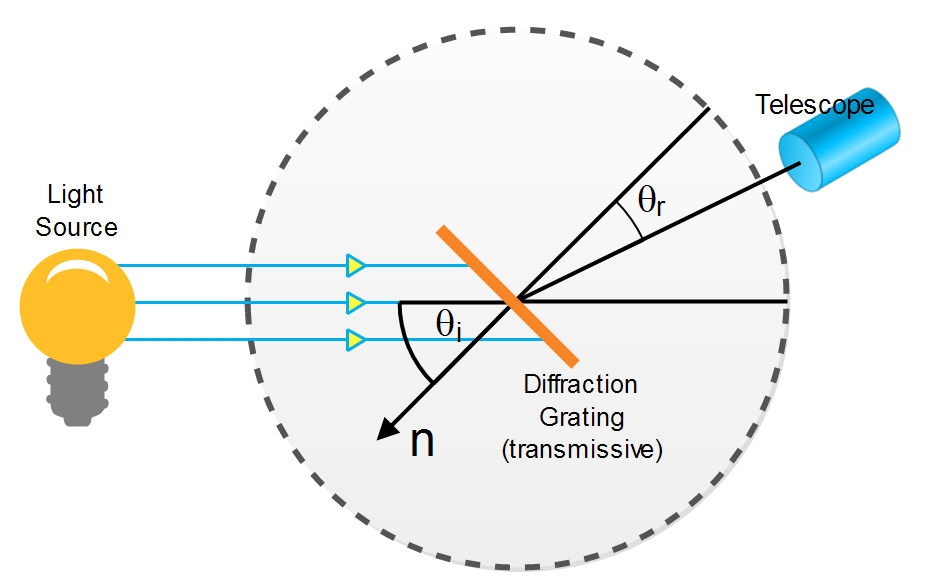
\includegraphics[scale=0.5]{evaluation/spectometer.png}
  \caption[Spectometer]{Spectometer: When a beam of monochromatic light passes through a grating placed in a spectrometer, images of the sources can be seen through the telescope at different angles.}
\label{fig:spectometer}
\end{figure}

Suppose an incident plane wavefront, composed of a monochromatic light source, is directed at a transmissive diffraction grating, parallel to its axis as shown in figure $\ref{fig:spectometer}$. Let the distance between successive slits on the grating be equal the value $d$. Furthermore, at a distance $L$, there is a screen parallel to the grating. Then the emitted waves will from a diffraction pattern on the screen which is the result of interference effects (constructively or destructively interference) among outgoing wavelets like shown in figure $\ref{fig:idealizedtransmissivegrating}$. 

\begin{figure}[H]
  \centering
  \subfigure[Idealized Transmissive Grating]{
    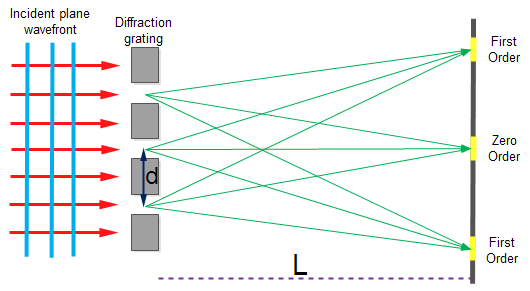
\includegraphics[scale=0.65]{evaluation/idealizeddiffgrating.png}
    \label{fig:idealizedtransmissivegrating}
  }
~  
  \subfigure[Parallel reflected Rays]{
    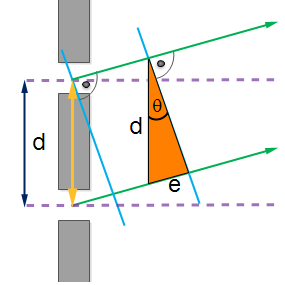
\includegraphics[scale=0.65]{evaluation/gratingsparallellines.png}
    \label{fig:gratingparallelreflectedrays}
  }

\caption[Idealized Diffraction Grating]{Light directed to parallel to grating}
\label{fig:lighthitsgrating}
\end{figure}

If the distance to the screen is much larger than the slits width, i.e. $L >> d$, then all the waves emanating from the surface and ending up at the receiver are parallel. Thus, the path difference between waves from any two adjacent slits can be derived by drawing a perpendicular line between the parallel waves. Applying simple trigonometry gives us this path difference as $e = d sin(\theta)$ as shown in figure $\ref{fig:gratingparallelreflectedrays}$. If the path difference equals one wavelength or a multiple of the wave's wavelength, the emerging, reflected waves from all slits will be in phase and a bright line will be observed at that point. Therefore, the condition for maxima in the interference pattern at the angle $\theta$ is: 

\begin{equation}
 d sin(\theta) = m \lambda 
\label{eq:simplegratingequation}
\end{equation}

where $m \in \mathds{N}_0$ is the order of diffraction. Because $d$ is very small for a diffraction grating, a beam of monochromatic light passing through a diffraction grating is split into very narrow bright fringes at large angles $\theta$. Without constraints of generality, either for a transmissive or a reflective diffraction grating type, an analogous derivation for equation $\ref{eq:simplegratingequation}$ can be derived.

\begin{figure}[H]
  \centering
  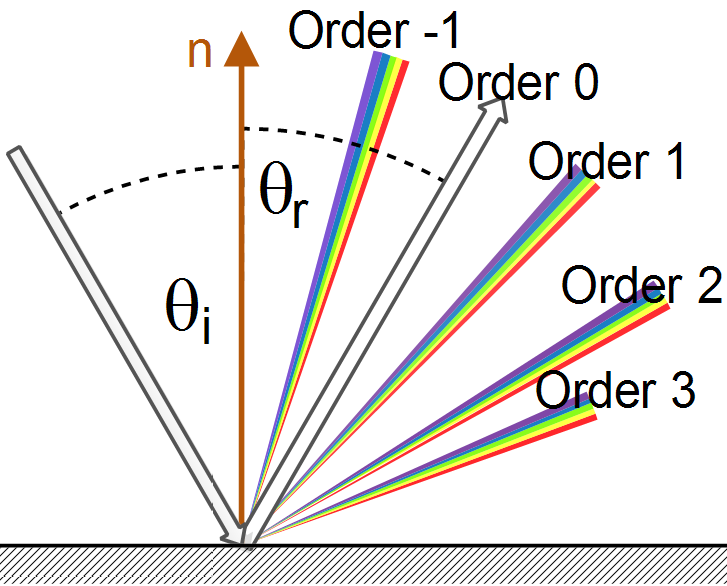
\includegraphics[scale=0.7]{evaluation/GratingSurface.png}
  \caption[Diffraction Orders]{Different$\footnotemark$ Orders of diffraction when light is diffracted on a reflective diffraction grating.}
\label{fig:gratingdiffractionorders}
\end{figure}
\footnotetext{This image has been taken from \\ \texttt{http://www.tau.ac.il/\textasciitilde phchlab/experiments\textunderscore new/SemB01\textunderscore Hydrogen/02TheoreticalBackground.html}}

When a beam of white light is directed at a diffraction grating along its axis, instead of a monochromatic bright fringe, a set of colored spectra are observed on both sides of the central white band. Figure $\ref{fig:diffractionslits}$ illustrates this for different number of slits on a diffraction grating. 

\begin{figure}[H]
  \centering
  \subfigure[one slit]{
    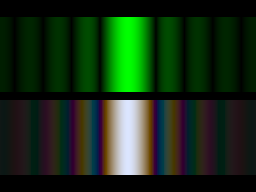
\includegraphics[scale=0.19]{evaluation/slits/spalt1.png}
    \label{fig:diffractionSlits1}
  }
  \subfigure[seven slits]{
    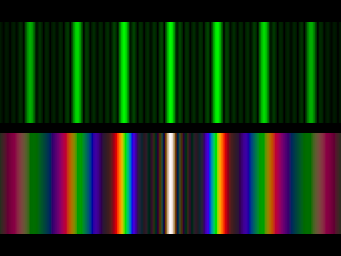
\includegraphics[scale=0.19]{evaluation/slits/spalt07.png}
    \label{fig:diffractionSlits7}
  }
  
\caption[N Slit Diffraction Grating Pattern]{Difference of diffraction pattern$\footnotemark$ between a monochromatic (top) and a white (bottom) light spectra for different number of slits.}
\label{fig:diffractionslits}
\end{figure}
\footnotetext{These images have been taken from \texttt{http://www.itp.uni-hannover.de/\textasciitilde zawischa/ITP/multibeam.html}}

Since the reflected angle $\theta_r$ increases with wavelength $\lambda$, red light, which has the longest wavelength, is diffracted through the largest angle. Similarly violet light has the shortest wavelength and is therefore diffracted the least. Thus, white light is split into its component colors from violet to red light. The spectrum is repeated in the different orders of diffraction, emphasizing certain colors differently, depending on their order of diffraction like shown in figure $\ref{fig:gratingdiffractionorders}$. Note that only the zero order spectrum is pure white.  
Figure $\ref{fig:nslitdiffractionintensity}$ shows the relative intensity resulting when a beam of light hits a diffraction grating for different number of periods. From the graph we recognise that the more slits a grating has, the sharper more slopes the function of intensity gets. This is similar like saying that, the more periods a grating has, the sharper the diffracted color spectrum gets like shown in figure $\ref{fig:diffractionslits}$. 

\begin{figure}[H]
  \centering
  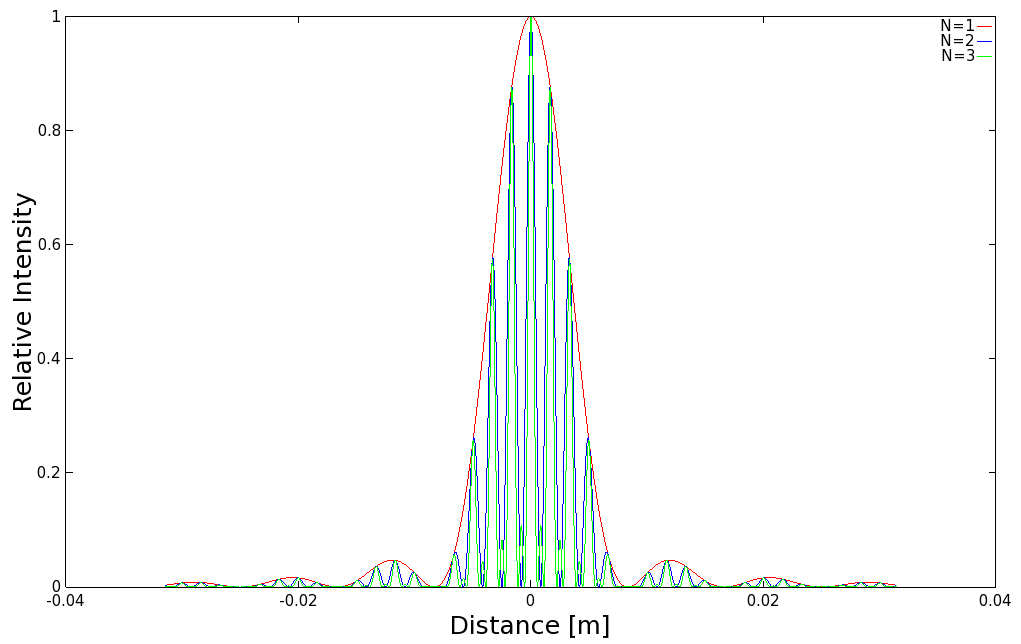
\includegraphics[scale=0.6]{evaluation/relativeintensivity.png}
  \caption[Intensity Plots for Different Number of Slits]{Relative intensities of a diffracted beam of light at wavelength $\lambda=500nm$ on a grating for different number of periods $N$ width slit width of 30 microns and slit separation of 0.15 mm each. The viewer is 0.5m apart from the grating.}
  \label{fig:nslitdiffractionintensity}
\end{figure}

\section{Verifications}
\label{sec:approachesverifications}
\begin{figure}[H]
  \centering
  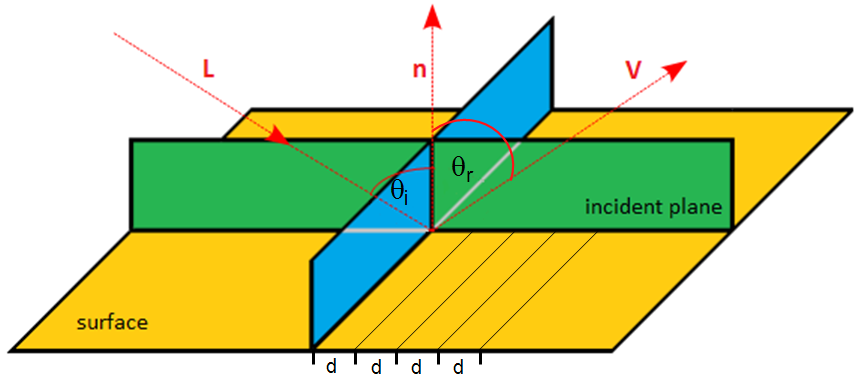
\includegraphics[scale=0.65]{evaluation/evalsetup2.png}
  \caption[Experimental Setup]{Experimental setup for evaluation: A light beam with direction $L$ hits the surface, representing a grating pattern with periodicity $d$, at the incident plane relative to the surface normal $n$ at angle $\theta_i$ and emerges at angle $\theta_r$ with viewing direction $V$.}
  \label{fig:experimentalsetup}
\end{figure}

The physical reliability of our BRDF models has been verified by applying it to a height field for a synthetic blazed grating. Figure $\ref{fig:experimentalsetup}$ illustrates the geometrical setup for our evaluation approach: A monochromatic beam of light with wavelength $\lambda$ hits a surface with periodicity $d$ at an angle $\theta_i$ relative to the normal $n$ along its incident plane. The beam emerges from the surface at the angle $\theta_r$ with certain intensity as predicted by our model. Note that actually two angles are necessary in order to define a direction vector, using spherical coordinates. However, in our evaluation we fixed the azimuthal angle of these directional vectors (Further information can be found in section $\ref{sec:evalprecomp}$). \\

In our evaluation we compare the local peak angles predicted by our model from those resulting by the grating equation. The grating equation models the relationship between the grating spacing, the incident light angle and the maximum angle for the diffracted light beams. 

\begin{figure}[H]
  \centering
  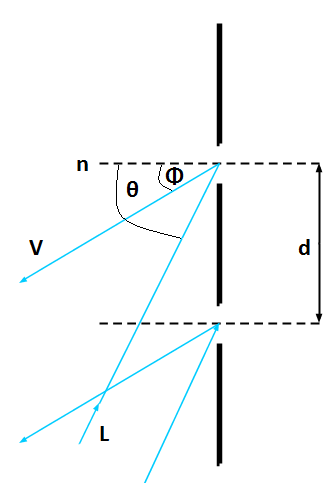
\includegraphics[scale=0.45]{evaluation/reflgrating.png}
  \caption[Reflective Grating]{Reflecting grating: When the incident light direction is not parallel to its axis at the grating, there is another $sin(\phi)$ involved. See also the grating equation $\ref{eq:gratingeq}$.}
  \label{fig:reflgrating}
\end{figure}

Figure $\ref{fig:reflgrating}$ shows that if the incident light is not along the axis of the diffraction gratings then it effects the optical path differences. The maximum in intensity is given by the grating equation derived from the equation $\ref{eq:simplegratingequation}$ following figure $\ref{fig:reflgrating}$: 

\begin{equation}
  sin(\theta_i) = sin(\theta_r) + \frac{m \lambda}{d}
\label{eq:gratingeq}
\end{equation}

In our evaluation we are interested in the first order diffraction, i.e. $m=1$. We further assume that the incident light direction $L$ is given. In contrast the direction of the reflected wave $V$ is a free parameter. \\

In Mathematics, a three dimensional direction vector is fully defined by two two angles, i.e. it can be represented by spherical coordinates with. Hence, $\theta_i$, is a given constant whereas $\theta_r$ is a free parameter for our evaluation simulation. Therefore, we are going to compare the maxima of the peak viewing angles corresponding to each wavelength using data produced by our method against the maxima resulting by the grating equation $\ref{eq:gratingeq}$.

\subsection{Numerical Comparisons}
\label{sec:evalprecomp}
In this section we explain how we evaluated the quality of our BRDF models. For a fixed incident light direction we want to compare the peak viewing angles with maximum reflectance of our methods with those resulting from the grating equation at different wavelengths. For this purpose we implemented the corresponding BRDF model for each of our shading approaches, FLSS, NMM and PQ, in Java. By fixing the azimuth angle$\footnote{Each direction vector in space can be expressed by spherical coordinates. Then, such a unit vector is defined by a pair of two angles, the inclination and the azimuth angle. For further information, please have a look at appendix $\ref{sec:sphericalcoordinates}$}$ of the incident light $L$- and viewing direction $V$, we reduced the degrees of freedom these directions, during our evaluation. Thus, any BRDF is then defined by function that expects as input arguments a wavelength $\lambda$ and the inclination angles of the incident light $\theta_i$ - and viewing direction $\theta_r$. The return value of such a function, denoted by $BRDF(\lambda, \theta_i, \theta_r)$, is the intensity value of the corresponding BRDF at these given input arguments. \\

In our evaluation program we set the incident light angle $\theta_i$ equal to $75 \degree$. This allows us to remove the argument $\theta_i$ from our BRDF function. Our java program computes each $BRDF$ function at a given discrete wavelength-viewing-angle grid, denoted by $[\Lambda, \Theta]$. The wavelength space $\Lambda = [\lambda_{min}, \lambda_{max}]$ and the viewing angle range $\Theta = [\alpha_{min}, \alpha_{max}]$ of our free parameter $\theta_r$ are discretized in equidistant steps whereas their step sizes. These step-sized, denoted by $(\lambda_{step}, \alpha_{step})$, are provided as input arguments for our Java evaluation program. \\

Next, let us have a closer look how our discrete $[\Lambda, \Theta]$ grid is constructed. The wavelength space $\Lambda$, which is ranging from $\lambda_{min}$ to $\lambda_{max}$, is discretized like the following:

\begin{equation}
\Lambda = \{\lambda = \lambda_{min} + k \cdot \lambda_{step} | k \in \{0,..,steps_{\lambda}-1\}\}
\label{eq:lambdaspacesetup}
\end{equation}

where $steps_{\lambda} = \frac{\lambda_{max}-\lambda_{min}}{\lambda_{step}}$.  We similarly discretise the viewing angle space $\Theta$ by setting an minimal and maximal viewing-angle boundary $\alpha_{min}$ and $\alpha_{max}$. Then $\ceil{\frac{\alpha_{max} - \alpha_{min}}{\alpha_{step}}}$ is the number of angles$ steps_{\alpha}$. And thus, our $\Theta$ space it defined like the following:

\begin{equation}
\Theta = \{\alpha = \alpha_{min} + k \cdot \alpha_{step} | k \in \{0,..,steps_{\alpha}-1\}\}
\label{eq:thetaspacesetup}
\end{equation}

Then, every BRDF java function is applied to the grid $[\Lambda, \Theta]$ and the resulting spectral response is stored in a matrix
\begin{equation} 
R = \{BRDF(\lambda_i, \theta_{r}^{j}) | i \in Index(\Lambda), \quad j \in Index(\Theta)\}
\label{eq:responsematrix}
\end{equation}

The generation process of the evaluation plots, which we discuss in section $\ref{sec:virtualtestbench}$, is described in algorithm $\ref{alg:evalmatlab}$. This algorithm takes the matrix R from equation $\ref{eq:responsematrix}$ as input argument. For the maximal reflectance of our methods at any wavelength, it computes the corresponding peak viewing angles and compares it to the angle resulting from the grating equation.

\begin{algorithm}[H]
\caption{BRDF Evaluation Graph Plotter}
\begin{table}[H]
  \begin{tabular}{@{}lll@{}}
    \textbf{Input:} & $R$ Matrix with $BRDF$ intensity values of $(\Lambda, \Theta)$ grid \\
    & $\Lambda$ discretized wavelength space used to compute $R$ \\
    & $(\alpha_{min})$ minimum value of viewing angle space $\Theta$ \\
    & $(\alpha_{step})$ discretization level of viewing angle space $\Theta$ \\
    & $d$ estimated periodicity of height field \\
    & $\theta_i$ fixed incident angle \\
    \textbf{Procedure:} & $getMaxIntensGridPointsOf(matrix,r):$ get the column-index of the largest  \\
    & \quad \quad \quad \quad \quad \quad \quad \quad \quad \quad \quad \quad \quad \quad \quad \quad \quad \quad intensity value in the row $matrix(r,*)$\\
    &$plotPoint(x,y)$: draw a point at $(x,y)$ \\
    \textbf{Output:} & Evaluation Plot of given BRDF model applied on given height field \\
  \end{tabular} 
\end{table}
\setlength{\fboxrule}{0pt} 
\begin{boxedminipage}{1.0\textwidth}
  \begin{algorithmic}[1]
    \ForAll{$\lambda_k \in \Lambda$}
      \State $\widetilde{\alpha} = getMaxIntensGridPointsOf(R, \lambda_k)$
      \Comment{$\widetilde{\alpha}$ $\equiv$ index viewing angle of max. R}
      \State $\widetilde{\alpha}_{r_k} = \alpha_{min} + \alpha_{step} \cdot \widetilde{\alpha}$
      \State $\theta_{r_k} = asin\left( \frac{\lambda}{d} - sin(\theta_i) \right)$
      \State $plotPoint(\lambda_k, \widetilde{\alpha}_{r_k})$
      \Comment{graph resulting by our BRDF model}
      \State $plotPoint(\lambda_k, \theta_{r_k})$
      \Comment{graph resulting by grating equation}
    \EndFor
  \end{algorithmic}
  \end{boxedminipage}
  \vskip1.5pt
\label{alg:evalmatlab}
\end{algorithm}

Algorithm $\ref{alg:evalmatlab}$ iterates over the wavelength space $\Lambda$ and generates our evaluation plots. For any wavelength it computes the viewing angle of the the maximal reflectance and the angle resulting from the grating equation as defined in equation $\ref{eq:gratingeq}$. Both angles are then plotted for the current wavelength in the current iteration. In the next section we will discuss the generated evaluation plots.

\subsection{Virtual Testbench}
\label{sec:virtualtestbench}
\begin{figure}[H]
  \centering
  \subfigure[Blazed Grating]{
    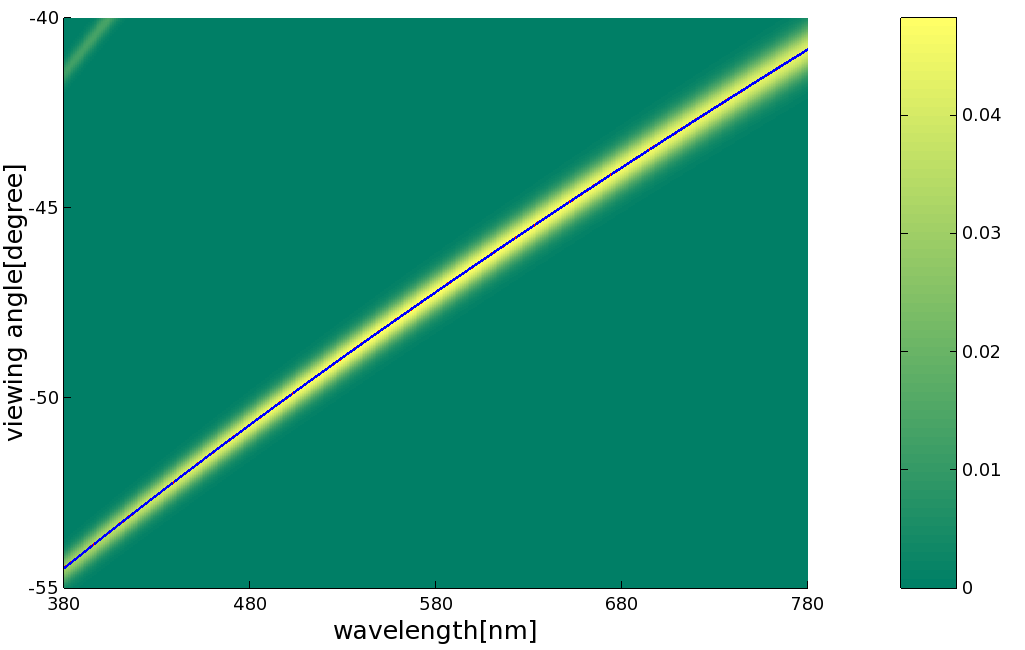
\includegraphics[scale=0.26]{evaluation/verification/flss_blazed.png}
    \label{fig:blazeval}
  }
~
  \subfigure[Xenopeltis Grating]{
    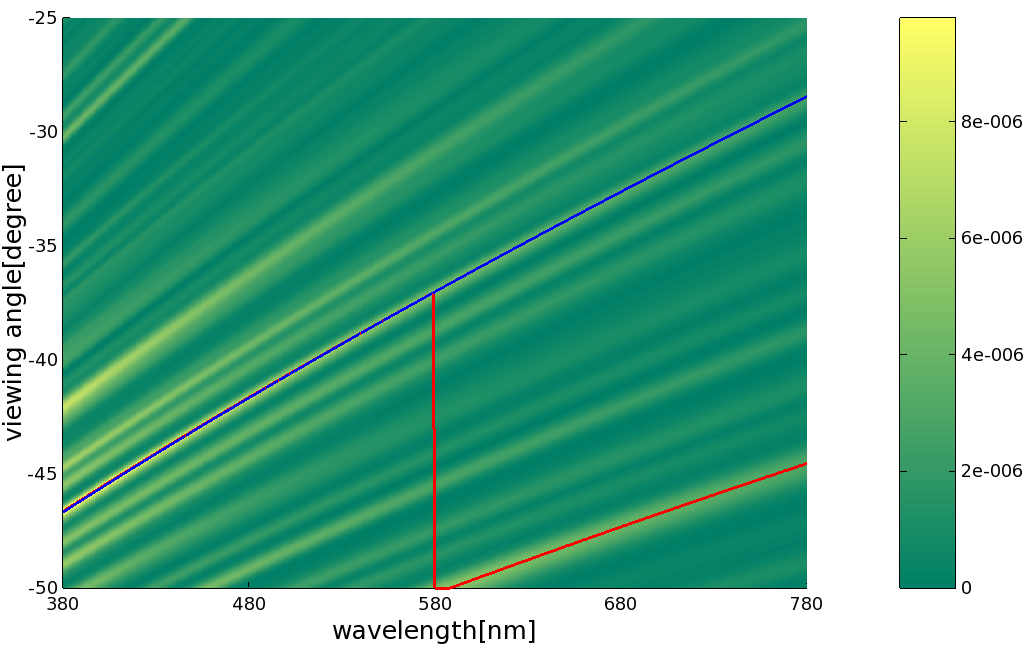
\includegraphics[scale=0.26]{evaluation/verification/flss_xeno.png}
    \label{fig:xenopeltiseval}
  }
  
\subfigure[Elaphe Grating]{
  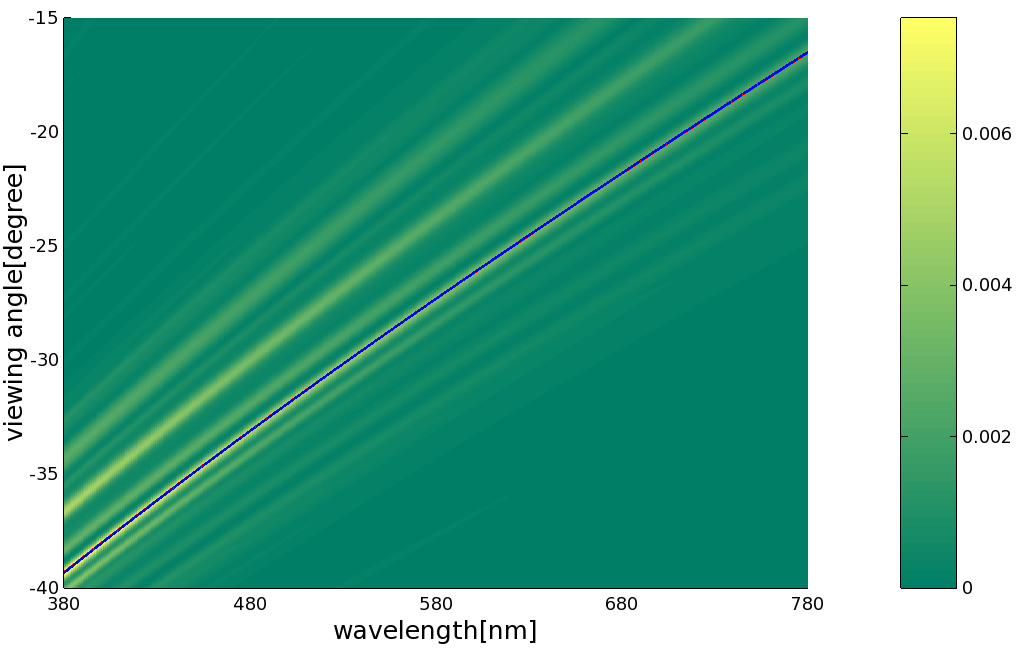
\includegraphics[scale=0.5]{evaluation/verification/flss_elaphe.png}
  \label{fig:elapheeval}
}

\caption[Validation of FLSS Approach applied on our Gratings]{Reflectance obtained by using the FLSS approach described in algorithm $\ref{alg:fragmentshaderall}$.}
\label{fig:evaluationdiffshaderalllambda}
\end{figure}

In this section we discuss the quality of our BRDF models applied to different surface structures. For that purpose we compare the resulting relative reflectance computed as described in section $\ref{sec:evalprecomp}$ for each of our BRDF models to the idealized grating equation $\ref{eq:gratingeq}$. 

\begin{table}[H]
\centering
\begin{tabular}{l|c|c|c|c|c|c|}
\cline{2-7}
                                         & \multicolumn{2}{c|}{FLSS} & \multicolumn{2}{c|}{NMM} & \multicolumn{2}{c|}{PQ} \\ \cline{2-7} 
                                         & mean        & variance    & mean        & variance   & mean       & variance   \\ \hline
\multicolumn{1}{|l|}{Blazed Grating}     & 2499.997    & 0.377       & 2499.997    & 0.377      & 2491.861   & 248.044    \\ \hline
\multicolumn{1}{|l|}{Elpahe Grating}     & 1144.262    & 0.401       & 1144.179    & 0.677      & 1052.308   & 49.678     \\ \hline
\multicolumn{1}{|l|}{Xenopeltis Grating} & 1552.27     & 0.45        & -           & -          & -          & -          \\ \hline
\end{tabular}
\caption[Estimated Grating Spacings]{Statistics of periodicity $d$ of our used gratings $\ref{fig:gratingpatches}$ estimated$\footnotemark$ by using the grating equation $\ref{eq:gratingeq}$.}
\label{tab:gratingsmeanvariance}
\end{table}
\footnotetext{This tabulated periodicity values are estimates similarly like described in the evaluation section of D.S.Dhillon's paper $\cite{daljitpaper}$.} 

Figure $\ref{fig:evaluationdiffshaderalllambda}$ shows the reflectance graphs resulting by the FLSS approach described in algorithm $\ref{alg:fragmentshaderall}$. This evaluation was applied to a idealized periodic structures, namely to the Blaze- $\ref{fig:blazeval}$ and to two natural gratings, the Elaphe- $\ref{fig:elapheeval}$ and Xenopeltis grating $\ref{fig:xenopeltiseval}$. For all our evaluation plots, we used an illumination angle of $\theta_i$ equal to $75\degree$. \\

Note that higher response values are plotted in yellow and lower values in green. For each of the graphs we determine the viewing angles with peak reflectance for each wavelength and then plot these peak viewing angles versus corresponding wavelengths as solid red curves. The blue curve represents diffraction angles for an idealized periodic structure with a certain periodicity $d$ according to the grating equation $\ref{eq:gratingeq}$. \\

By rearranging the terms of the grating equation defined in equation $\ref{eq:gratingeq}$ and using the peek reflectance angle $\theta_{r_k}$ derived like in algorithm $\ref{alg:evalmatlab}$ using the matrix R of equation $\ref{eq:responsematrix}$, we can compute a periodicity vale $d_k$ for any wavelength $\lambda_k$.  
\begin{equation}
  d_k = \frac{\lambda}{sin(\theta_{r_k}) + sin(\theta_i)}
\end{equation}

By computing the mean value of these $d_k$ values for all $\lambda$ in $\Lambda$ we can compute an estimated periodicity value $d$. We estimated these periodicity values for every grating structure and every method we are using. Thes corresponding periodicity values tabulated in table $\ref{tab:gratingsmeanvariance}$. \\

The red and blue curve are closely overlapping in our figures $\ref{fig:blazeval}$ and $\ref{fig:elapheeval}$. For Blaze and Elaphe there is only diffraction along only along one direction perceivable. Since the Blazed grating is synthetic we use its exact periodicity to plot the blue curve instead of estimating it. The Xenopeltis grating is evaluated just along the direction for the finger like structures. For Xenopeltis it is interesting to see that the red curve for the peak viewing angle toggles between two ridges corresponding to two different periodicities. this happens because there are multiple sub regions of the nanostructure with slightly different orientations and periodicity. Each sub region carves out a different yellowish ridge. depending on the viewing angle, reflectance due to one such subregion can be higher than from the others. \\

Figure $\ref{fig:evaluationdiffshadernminmax}$ shows the evaluation plots for the NMM approach applied to the Blazed- (see figure $\ref{fig:elapheneval}$) and the Elaphe-grating (see figure $\ref{fig:elapheneval}$). The NMM approach is an optimization of the FLSS approach and is discussion in section $\ref{sec:nmmapproach}$. The response curve of each plotted NMM approach graph closely matches the corresponding grating equation curve. Furthermore, the evaluation graphs of the NMM approach look similar to the corresponding evaluation plots of the FLSS approach shown in figure $\label{ref:evaluationdiffshaderalllambda}$. Thus, this confirms that the NMM optimization works well.

\begin{figure}[H]
  \centering
  \subfigure[Blaze grating]{
    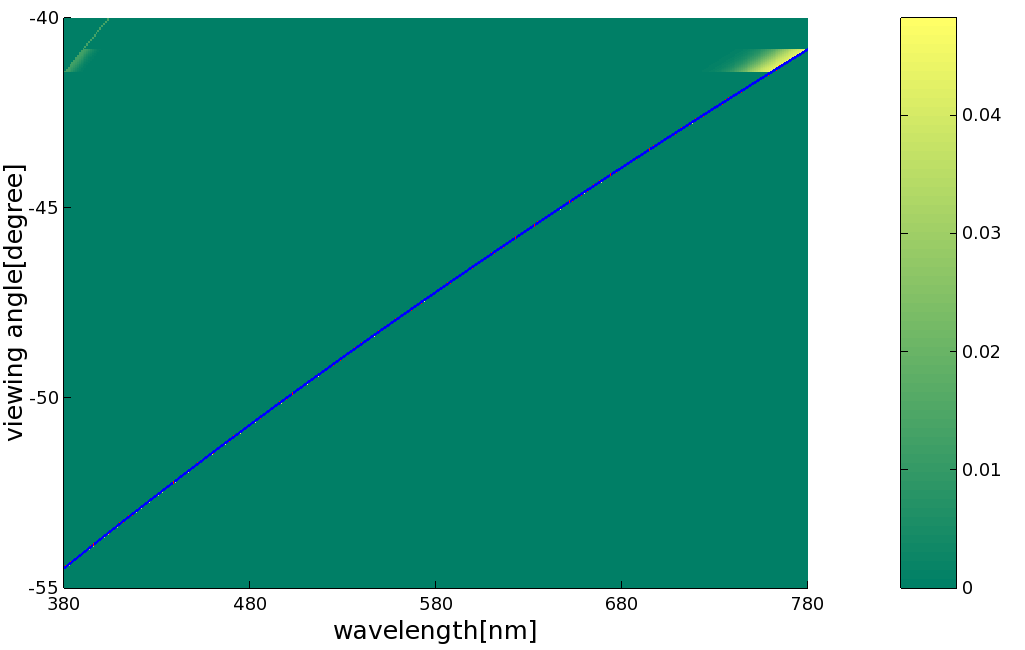
\includegraphics[scale=0.26]{evaluation/verification/nmm_blazed.png}
    \label{fig:blazneval}
  }
~
  \subfigure[Elaphe grating]{
    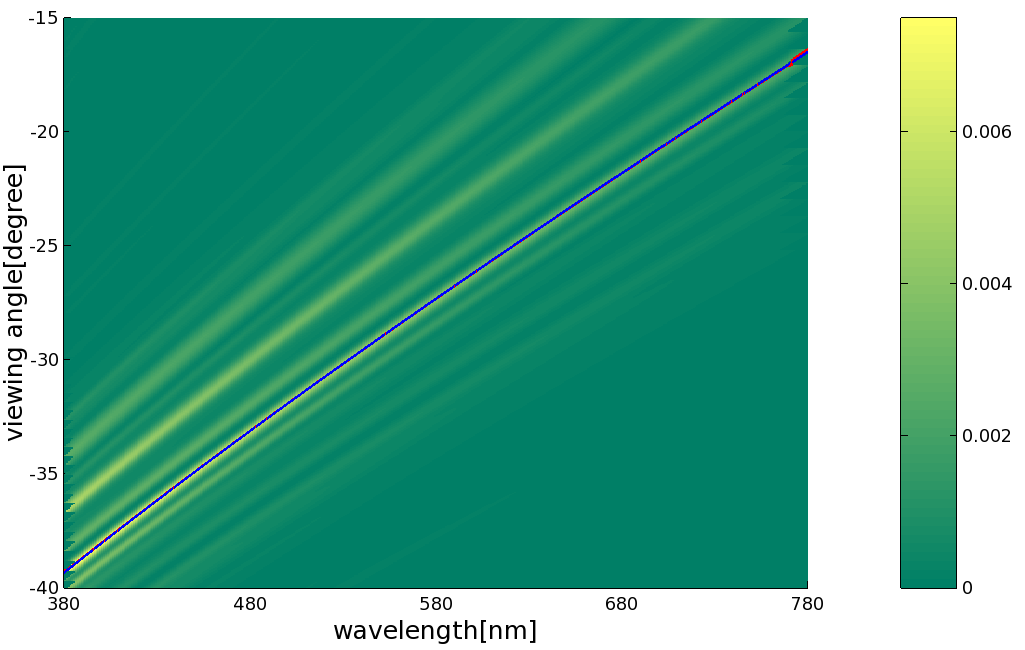
\includegraphics[scale=0.26]{evaluation/verification/nmm_elaphe.png}
    \label{fig:elapheneval}
  }
\caption[Validation of NMM Approach applied on our Gratings]{Reflectance obtained using NMM optimization apporach.}
\label{fig:evaluationdiffshadernminmax}
\end{figure}

Last, let us consider the evaluation graphs in figure $\ref{fig:evaluationdiffshaderpq}$ for the PQ approach described in algorithm $\ref{alg:sincinterpolation}$. The PQ approach assumes the given grating being periodically distributed on the surface of a shape. For this approach we have plotted evaluation graphs of the Blaze- (See figure $\ref{fig:blazepqeval}$) and Elaphe grating (See figure $\ref{fig:elaphepqeval}$). The response curves of both PQ evaluation graphs exhibit some similarities, but also some differences, compared to their corresponding grating equation curve. We could say that the response curve of the blaze grating is weakly oscillating around the grating equation curve (blue), but basically following it even there are some outliers. The response curve of the Elpahe grating is not following its corresponding first order grating equation curve well. This could be due to the PQ's assumption that a given height field has to be periodically distributed along the surface. But in general, for natural gratings, this is assumption does usually not hold true. Nevertheless, the red curve fits one of the response curves. We conclude that the PQ approach will produce not accurate results compared to the FLSS approach. Thus, the PQ approach is sub-optimal.

\begin{figure}[H]
  \centering
  \subfigure[Blaze grating]{
    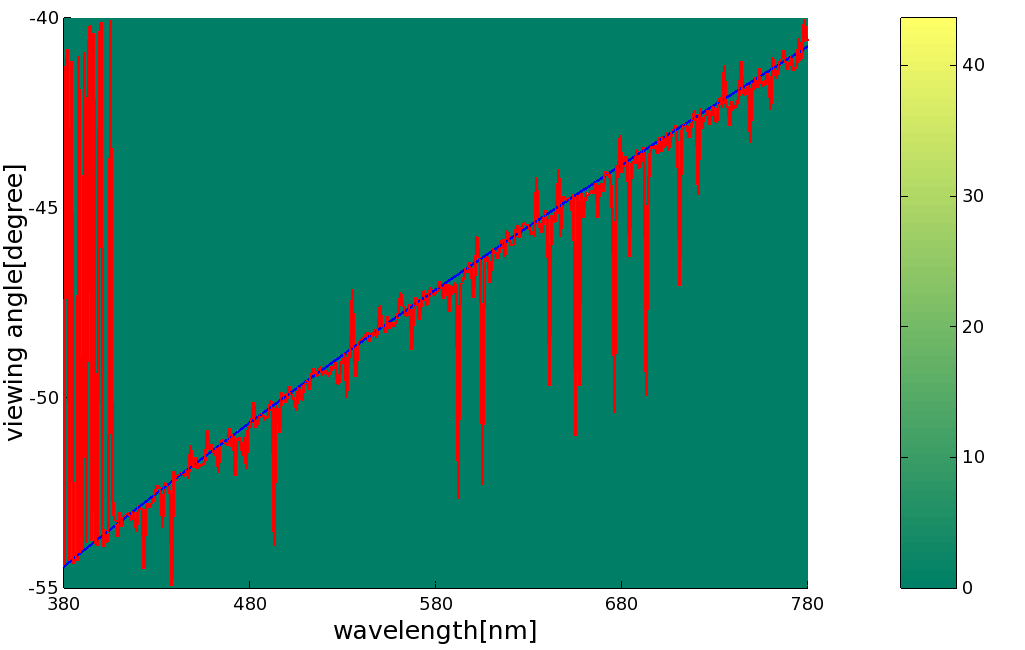
\includegraphics[scale=0.26]{evaluation/verification/pq_blazed.png}
    \label{fig:blazepqeval}
  }
~
  \subfigure[Elaphe grating]{
    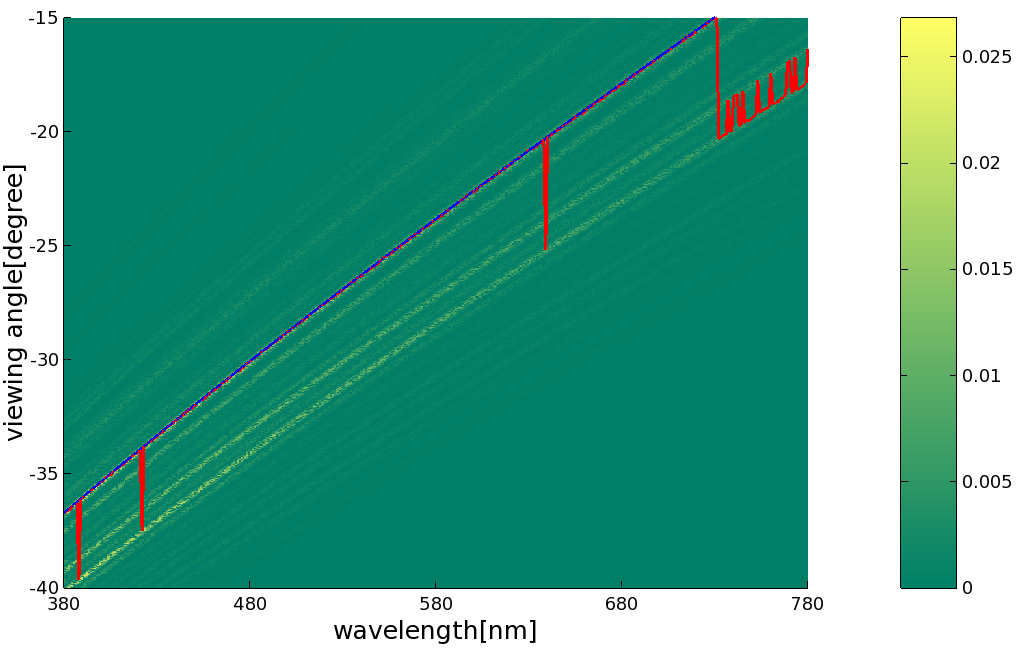
\includegraphics[scale=0.26]{evaluation/verification/pq_elaphe.png}
    \label{fig:elaphepqeval}
  }
\caption[Validation of PQ Approach applied on our Gratings]{Reflectance obtained using PQ optimization approach.}
\label{fig:evaluationdiffshaderpq}
\end{figure}
